% -*- latex -*-
%%%%%%%%%%%%%%%%%%%%%%%%%%%%%%%%%%%%%%%%%%%%%%%%%%%%%%%%%%%%%%%%
%%%%%%%%%%%%%%%%%%%%%%%%%%%%%%%%%%%%%%%%%%%%%%%%%%%%%%%%%%%%%%%%
%%%%
%%%% This text file is part of the source of 
%%%% `Parallel Programming in MPI and OpenMP'
%%%% by Victor Eijkhout, copyright 2012-2023
%%%%
%%%% mpi-commsplit.tex : about splitting communicators
%%%%
%%%%%%%%%%%%%%%%%%%%%%%%%%%%%%%%%%%%%%%%%%%%%%%%%%%%%%%%%%%%%%%%
%%%%%%%%%%%%%%%%%%%%%%%%%%%%%%%%%%%%%%%%%%%%%%%%%%%%%%%%%%%%%%%%

\Level 0 {Splitting a communicator}
\label{sec:comm-split}

Above we saw several scenarios where it makes sense to divide
\lstinline{MPI_COMM_WORLD} into disjoint subcommunicators.
The command \indexmpiref{MPI_Comm_split} uses a `color' to define
these subcommunicators:
all processes in the old communicator with the same color
wind up in a new communicator together. The old communicator still exists,
so processes now have two different contexts in which to communicate.

The ranking of processes in the new communicator is determined by a `key' value:
in a subcommunicator the process with lowest key is given the lowest rank, et cetera.
Most of the time, there is no reason to use a relative ranking that is different from
the global ranking, so the \indexmpishow{MPI_Comm_rank} value of the global communicator
is a good choice.
Any ties between identical key values are broken by using the rank from the original
communicator.
Thus, specifying zero as the key will also retain the original process ordering.

\begin{figure}[ht]
  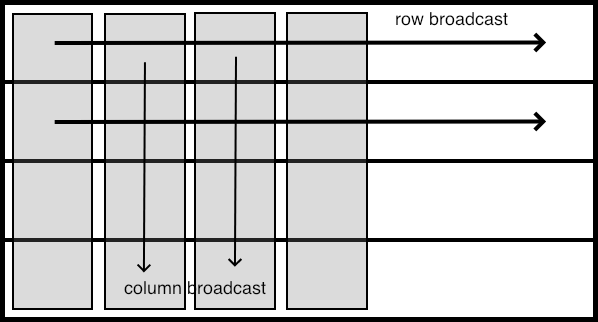
\includegraphics[scale=.4]{procgrid-bcast}
  \caption{Row and column broadcasts in subcommunicators}
  \label{fig:procgrid-bcast}
\end{figure}

Here is one example of communicator splitting. Suppose your processors
are in a two-dimensional grid:
\begin{lstlisting}
MPI_Comm_rank( MPI_COMM_WORLD, &mytid );
proc_i = mytid % proc_column_length;
proc_j = mytid / proc_column_length;
\end{lstlisting}
You can now create a communicator per column:
\begin{lstlisting}
MPI_Comm column_comm;
MPI_Comm_split( MPI_COMM_WORLD, proc_j, mytid, &column_comm );
\end{lstlisting}
and do a broadcast in that column:
\begin{lstlisting}
MPI_Bcast( data, /* stuff */, column_comm );
\end{lstlisting}
Because of the SPMD nature of the program, you are now doing in parallel
a broadcast in every processor column. Such operations often appear
in \indexterm{dense linear algebra}.

\begin{exercise}
  \label{ex:rowcolcomm}
  Organize your processes in a grid, and make subcommunicators for
  the rows and columns. For this compute the row and column number of
  each process.

  In the row and column communicator, compute the rank. For instance,
  on a $2\times3$ processor grid you should find:
\begin{verbatim}
Global ranks:  Ranks in row:  Ranks in colum:
  0  1  2      0  1  2        0  0  0
  3  4  5      0  1  2        1  1  1
\end{verbatim}

  Check that the rank in the row communicator is the column number,
  and the other way around.

  Run your code on different number of processes, for instance a
  number of rows and columns that is a power of~2, or that is a prime number.
\begin{tacc}
    This is one occasion where you could use \n{ibrun -np 9};
    normally you would \emph{never} put a processor count on \n{ibrun}.
\end{tacc}
  \skeleton{procgrid}
\end{exercise}

\begin{pythonnote}{Comm split key is optional}
  In Python, the `key' argument is optional:
  %
  \psnippetwithoutput{commsplitp}{examples/mpi/p}{dup}
\end{pythonnote}

\begin{mplnote}{Communicator splitting}
  \label{mpl::split}
  In \ac{MPL}, splitting a communicator is done as one of the overloads
  of the communicator constructor;
  %
  \cxxverbatimsnippet[examples/mpi/mpl/commsplit.cxx]{commsplitmpl}

  \begin{mplimpl}
    The \lstinline+communicator::+\indexmpldef{split} identifier
    is an object of class
    \lstinline+communicator::+\indexmpldef{split_tag},
    itself is an otherwise empty
    subclass of \indexmplshow{communicator}:
\begin{lstlisting}
class split_tag {};
static constexpr split_tag split{};
\end{lstlisting}
  \end{mplimpl}
\end{mplnote}


There is also a routine \indexmpishow{MPI_Comm_split_type}
which uses a type rather than a key to split the communicator.
We will see this in action in section~\ref{mpi-comm-split-type}.

As another example of communicator splitting, consider the recursive
algorithm for \indextermbus{matrix}{transposition}.
%
\index{transpose!recursive}
%
Processors are organized in a square grid. The matrix is divided
on $2\times 2$ block form.

\begin{exercise}
  \label{ex:recursivetranspose}
  Implement a recursive algorithm for matrix transposition:
  
  \includegraphics[scale=.06]{recursive-transpose}

  \begin{itemize}
  \item Swap blocks $(1,2)$ and $(2,1)$; then
  \item Divide the processors into four subcommunicators, and
    apply this algorithm recursively on each;
  \item If the communicator has only one process, transpose the matrix in place.
  \end{itemize}
  (assume one element per process)
\end{exercise}

